\section{Effective Differentially Private Fine-Tuning}
By studying the impact of hyperparameters and choice of fine-tuning objective, we demonstrate that the performance of the DP-Adam baseline can be substantially improved, even matching some strong non-private learning results.
Our analyses reveal common failure modes when straightforwardly applying DP optimization and explain poor results reported in past works that consider these baselines.


\subsection{Hyperparameter Tuning}\label{sec:good_hyper_params}
DP optimization is sensitive to the choice of hyperparameters~\citep{papernot2019making}.
Our experiments suggest that its performance can vary from being close to that of random initialization with ill-chosen hyperparameters to near state-of-the-art with appropriately chosen ones. As a consequence, we present simple but effective guidelines on setting the most important hyperparameters.
Unless otherwise stated, the unmentioned hyperparameters are set to defaults documented in Appendix~\ref{app:good_hyper_params}. 

\subsubsection{Batch Size, Learning Rate \& Training Epochs}
Our experiments suggest that batch size is one of the most important hyperparameters to set correctly, and the dependence of the optimal batch size on the learning rate and training epochs makes its selection complex.
We first describe batch size selection in realistic, compute-bound settings and then describe how the complexity of identifying the optimal batch size in these situations arise due to constraints on the number of training epochs.

\begin{wrapfigure}[20]{r}{0.5\textwidth}
\centering
\vspace{-2mm}
{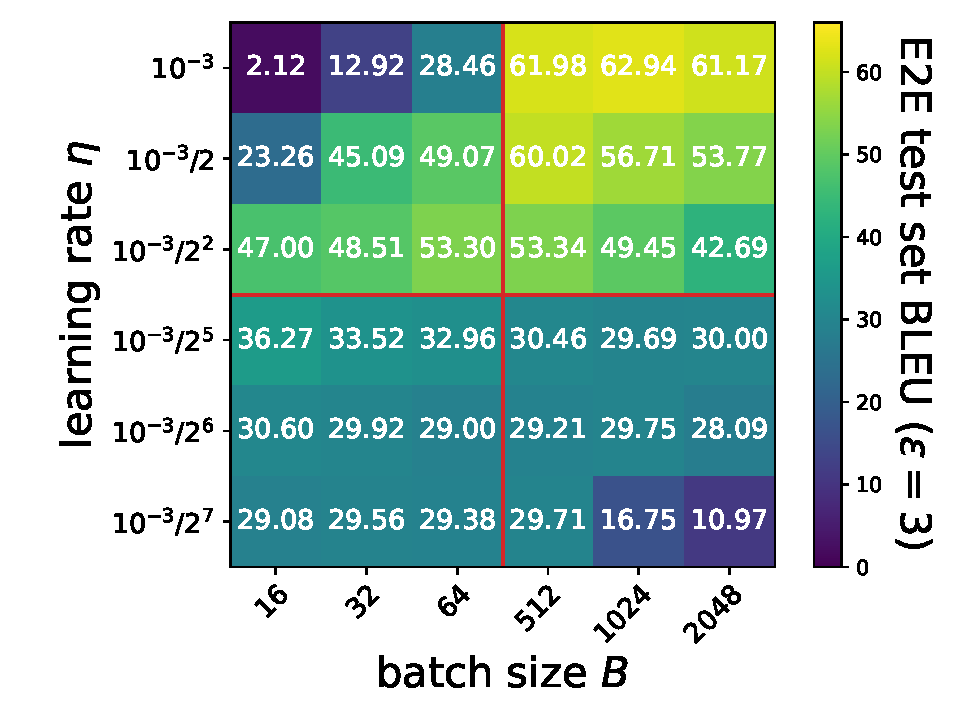
\includegraphics[width=0.45\textwidth]{figs/bs_vs_lr_BLEU.pdf}}
\caption{
Large batches and learning rates lead to good performance when the number of epochs is fixed.
Red lines divide heat map into four panels. Top and bottom correspond to low and high learning rate regimes; left and right correspond to small and large batch regimes.
Numbers are BLEU scores on the test split of E2E; higher is better.
}
\label{fig:bs_vs_lr}
\end{wrapfigure}
\paragraph{Fixed Training Epochs $E$.}
We first describe a very practical situation in which there is a constraint on the compute budget.
For the case of DP-SGD, this compute budget constraint often loosely translates to a constraint on the number of examples processed for gradient updates.\footnote{This is because DP-SGD often necessitates microbatching, in which case the number of backward passes is independent of the actual batch size for gradient updates but dependent on numbers of passes through the data.} 
In this fixed training epoch setting, the learning rate and batch size jointly affect performance, since using larger batches implies performing fewer gradient updates. 
To study this joint influence empirically, we fine-tune GPT-2 on the E2E dataset for table-to-text generation with DP-Adam at $\epsilon=3$ with various batch sizes and learning rates. 
Figure~\ref{fig:bs_vs_lr} shows that the best performing models (BLEU score \mytextapprox 62)
are obtained with both a large batch size and large learning rate. 
Using a small learning rate together with a small batch size yields considerably worse results. 
Note a seq2seq baseline achieves a test 
BLEU of \mytextapprox 65 without privacy here~\citep{wiseman2018learning}. 

Recall that in the non-private world, pretrained language models are typically fine-tuned with small batch sizes and small learning rates with Adam (bottom left panel in Figure~\ref{fig:bs_vs_lr}).
This implies that na\"ively fine-tuning pretrained language models privately using hyperparameters routinely used for non-private learning would degrade performance by more than necessary.\footnote{Anecdotally, moderately large learning rates also tend to work reasonably well in non-private learning. Small learning rates, however, are generally more stable, especially when (average) gradients aren't clipped.}

Recently, \cite{tramer2020differentially} studied how the batch size and learning rate jointly affect learning private image classifiers while holding other hyperparameters fixed.
They heuristically suggested a \textit{linear scaling rule}: Scaling the learning rate together with the batch size by the same constant should yield models with almost the same performance. 
However, Figure~\ref{fig:bs_vs_lr} indicates that this fails to hold consistently as it falsely predicts that large batch and high learning rate (top right entry) would have equal performance to small batch and low learning rate (bottom left entry).
We explain why linear scaling fails to predict performance for the small batch regime in Appendix~\ref{app:linear_scaling}. 

\paragraph{Fixed Update Steps $S$.}
In the fixed epoch setting, we saw that the optimal batch size was complex due to the trade-off between batch size and number of gradient updates.
We now show that the complexity of setting batch sizes arises almost entirely from this tradeoff by considering a different setting, where the total number of gradient updates (rather than epochs) is fixed.
In this case, using larger batches implies training for more epochs.

Here, we find that using larger batch sizes almost always results in better performance at a given privacy budget at the cost of processing more examples with more compute, once the other hyperparameters $S$, $\eta$, $C$, $\epsilon$, and $\delta$ are fixed.
We provide a heuristic explanation of this by introducing the idea of an \textit{effective noise multiplier} $\sigma_{\text{eff}} = \tfrac{\sigma}{q} = \tfrac{\sigma N} {B}$.  
Recall the noise multiplier $\sigma$ is determined from the privacy budget $(\epsilon, \delta)$, the number of update steps $S$, and the sampling rate $q$. 
In addition, recall the privatized gradient $\bar{g}$ in DP-SGD/DP-Adam which loosely takes the following form:
\eq{
\label{eq:sigma_eff_intuition}
	\bar{g} = \widetilde{g} + \widebar{z}
	, \quad
	\widetilde{g} = \frac{1}{B} \sum_{i \in \mathcal{B}} \text{Clip}(\nabla \mathcal{L}_i, C), \quad
	\widebar{z} \sim \mathcal{N} \Big(0, C^2 \tfrac{ \sigma^2}{B^2} I_p \Big) = \mathcal{N} \Big( 0, C^2 \tfrac{\sigma_{\text{eff}}^2}{N^2} I_p \Big),
}
where $\mathcal{B}$ is the Poisson-sampled batch of indices, $\nabla \mathcal{L}_i$ is the gradient of the $i$th example and $\text{Clip}(v, C) = v \cdot \min(1, \nicefrac{C}{\normtwo{v}} )$ clips the vector $v$ by the norm constraint $C$. 
We observe that for moderately large batches, the signal-to-noise ratio 
$r = \nicefrac{\normtwo{\widetilde{g}}}{\normtwo{\widebar{z}}}$ is mainly controlled by the batch size through the effective noise multiplier: 
The signal term $\widetilde{g}$ tends to concentrate quickly due to being an average of bounded vectors, whereas the effective noise multiplier $\sigma_{\text{eff}}$ decreases as the batch size $B$ increases (shown in Figure~\ref{fig:batch_size_fixed_t} (a)).
Figure~\ref{fig:batch_size_fixed_t} (b) plots the average signal-to-noise ratio $\widebar{r}$ over the first 30 gradient updates against the final model's performance on E2E and demonstrates that large batches (up to a threshold) correlates with both increased signal-to-noise ratio at the beginning of training and better performance at the end of training.
These findings additionally resonate with and explains recent empirical successes of large-scale private pretraining~\citep{anil2021large}.
\begin{figure}[htb]
\begin{center}
\begin{minipage}[t]{0.48\linewidth}
\centering
{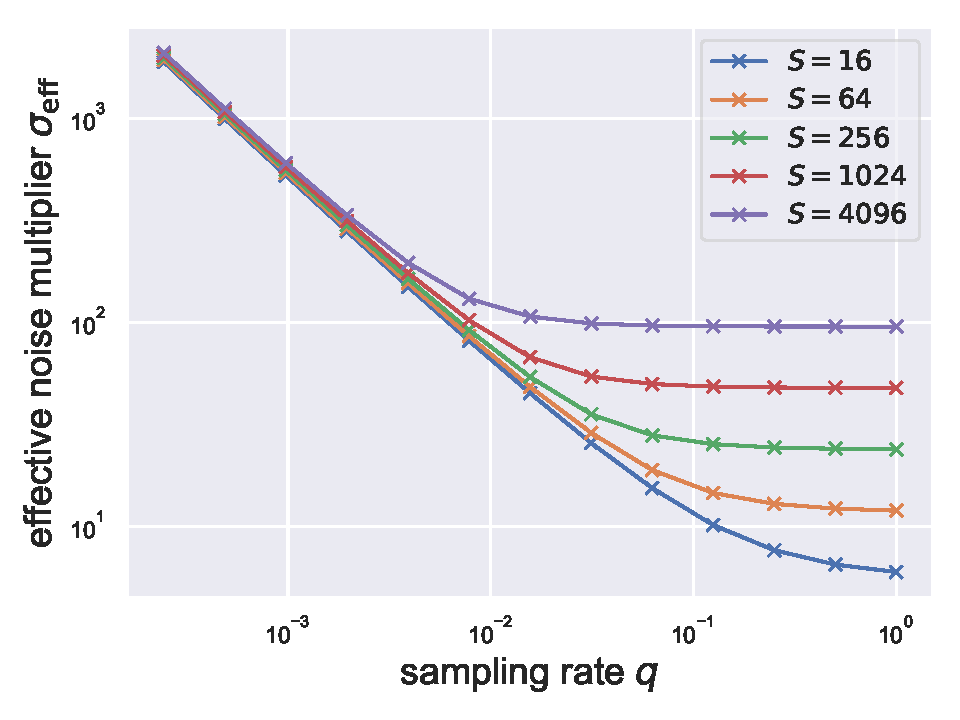
\includegraphics[width=0.98\textwidth]{figs/fixed_t_q_vs_sigma_eff_3.pdf}}
\end{minipage}
\begin{minipage}[t]{0.48\linewidth}
\centering
{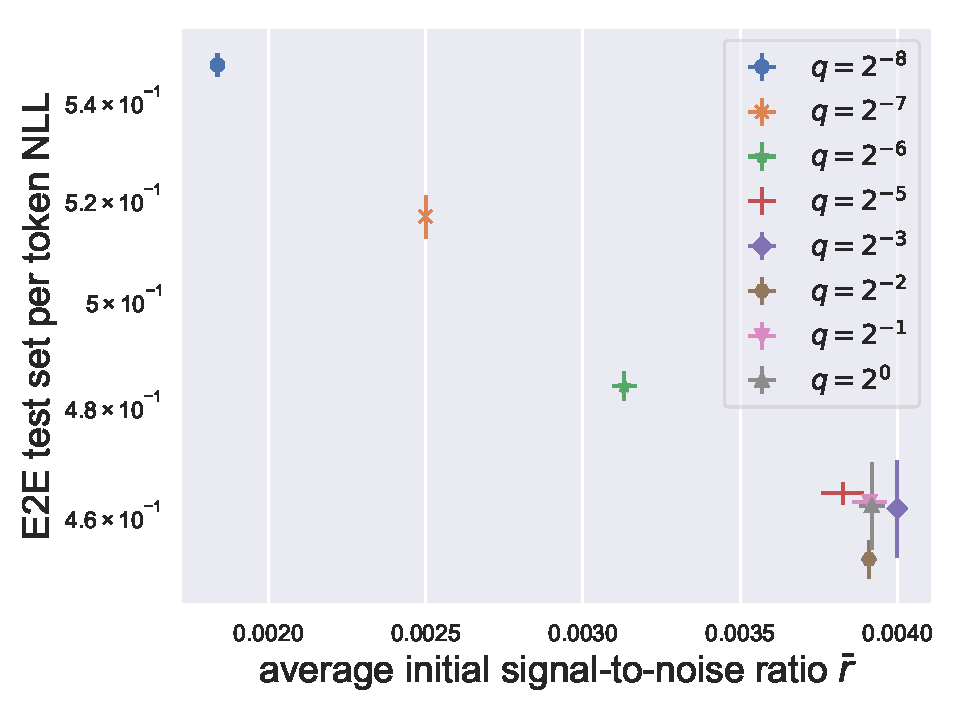
\includegraphics[width=0.98\textwidth]{figs/snr_vs_test_xent.pdf}}
\end{minipage}
\end{center}
\caption{
\textbf{Left:} Effective noise multiplier decreases with increasing sampling rate for various fixed number of updates $S$.
\textbf{Right:} Large batch sizes (corresponding to large $q$ in the figure) have higher signal-to-noise ratio at the beginning of training, which log-linearly correlates with final performance.
}
\label{fig:batch_size_fixed_t}
\end{figure}



\subsubsection{Clipping Norm}
DP optimization is known to be sensitive to the choice of clipping norm.
Since the scale of noise depends on this clipping norm (recall its standard deviation is $C \sigma$), picking the threshold $C$ much larger than the actual gradient norm implies more noise is being applied than necessary.
In practice, we have found that a small clipping norm which enforces almost all gradients to be clipped throughout training leads to the best performing models; see Figure~\ref{fig:app_hyperparameter}.

\begin{figure}[H]
\begin{center}
\begin{minipage}[t]{0.48\linewidth}
\centering
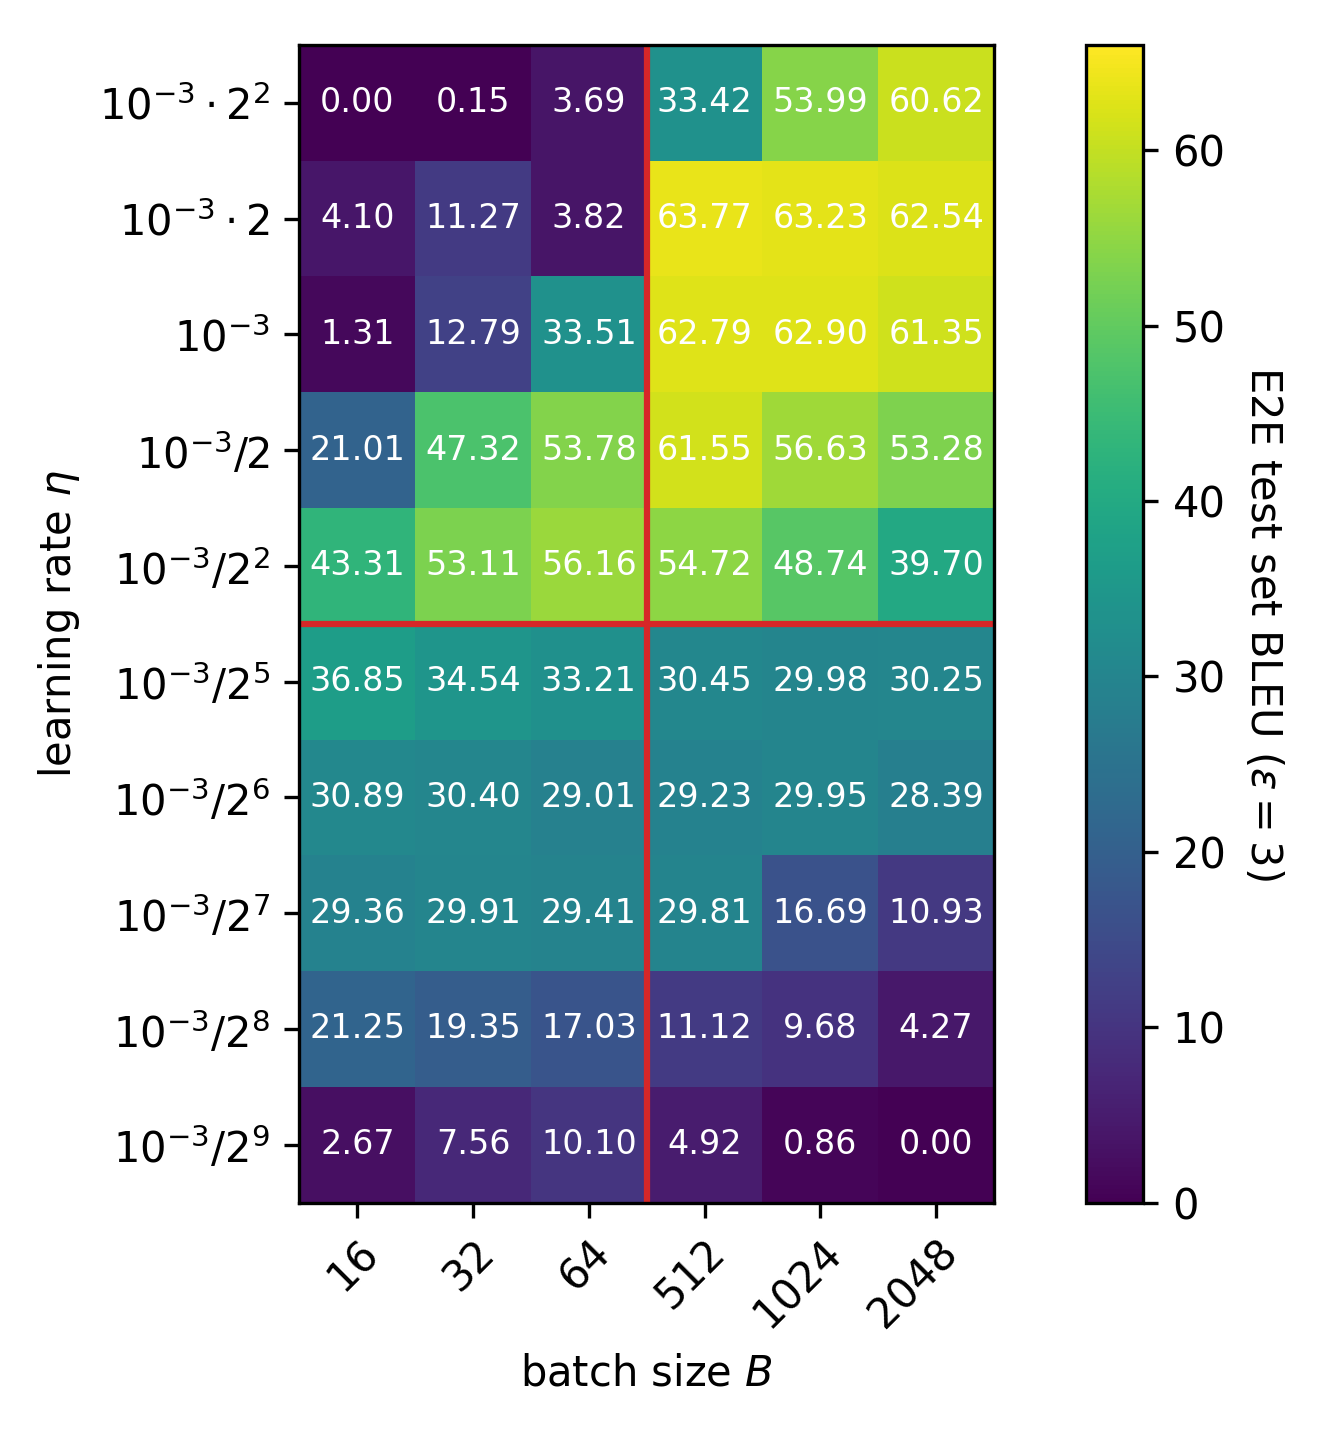
\includegraphics[width=0.96\textwidth]{figs/bs_vs_lr_BLEU_v2_cropped.png} \\ \vspace{-0.10cm}
(a) Batch size.
\end{minipage}
\begin{minipage}[t]{0.48\linewidth}
\centering
{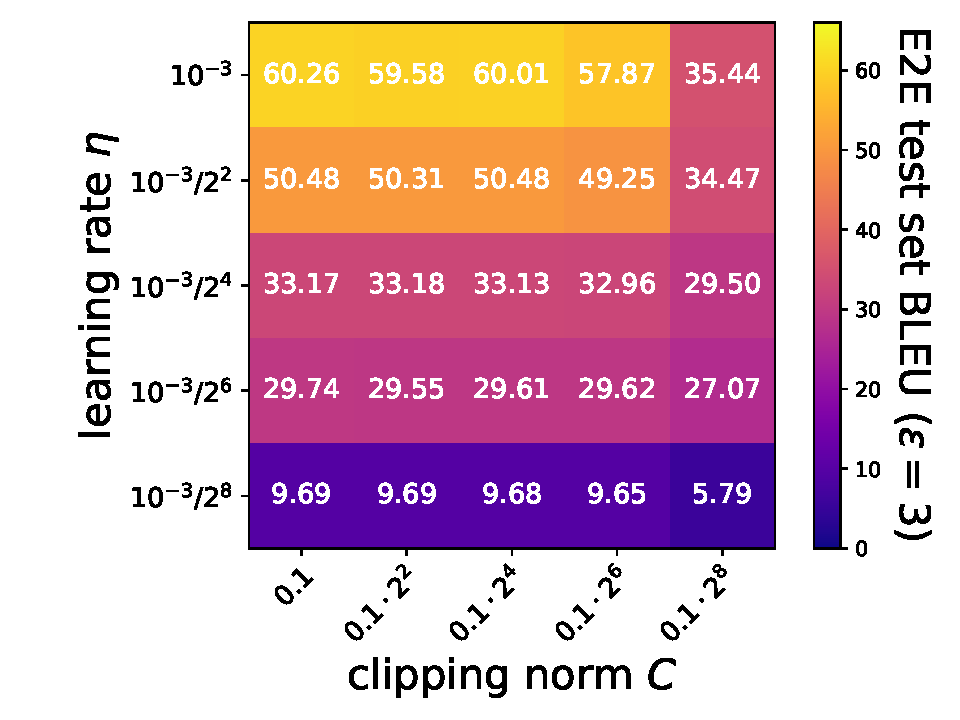
\includegraphics[width=0.96\textwidth]{figs/cn_vs_lr_BLEU.pdf}} \\ \vspace{-0.10cm}
(b) Clipping norm. 
\end{minipage}
\end{center}
\caption{Additional results on hyperparameter sensitivity.}
\label{fig:app_hyperparameter}
\end{figure}


\subsection{Improving the task alignment helps private learning}\label{sec:task_alignment}
Our fine-tuned models on language generation tasks work well since the pretraining objective and downstream task are \emph{aligned}: Both involve predicting sequences of tokens.
This alignment simplifies the task and benefits private learning. 
While pretrained models are naturally aligned for language generation, it is much less so for classification tasks. The standard approach for adapting language models for classification involves stacking a freshly initialized network on top of the encoding of the special \texttt{[CLS]} token and jointly optimizing all parameters~\citep{devlin2018bert}. 
This workflow introduces a discrepancy between pretraining and fine-tuning: Pretraining predicts masked out words from a large vocabulary whereas fine-tuning predicts integer labels.

To eliminate the discrepancy, we instead consider learning to predict the missing word during fine-tuning for classification. 
For example, for sentiment classification, we reframe the problem as filling in the \texttt{[MASK]} token in the sequence ``\texttt{<INPUT>}. It is \texttt{[MASK]}.'' and compare the probabilities of words ``awesome'' and ``terrible''.
This text infilling task is almost exactly the procedure used for pretraining masked language models, and recent works have demonstrated its effectiveness for knowledge probing~\citep{petroni2019language}, few-shot learning~\citep{gao2020making} and multi-task fine-tuning~\citep{wei2021finetuned}. 
On SST-2, we found that using the generic template as described above already improved private fine-tuning performance by $3\sim5\%$ across different settings.
Table~\ref{table:glue} (to be presented) contains additional results and Appendix~\ref{app:task_alignment} includes analyses on choices of label words.

